\item
  Out of a group of 40 students all play at least one of badminton, volleyball or table tennis.
  \begin{itemize}
    \item 8 students play all three games, 10 students play badminton and table tennis.
    \item 20 students play table tennis and volleyball, 12 students play badminton and volleyball.
    \item 30 students play table tennis, 25 students play volleyball.
  \end{itemize}
  \begin{enumerate}
    \item
      Draw a Venn diagram of the situation.
    \item
      How many of the students play \emph{only} badminton?
    \item
      How many of the students play badminton?
    \item \label{marginal}
      Assume one student is picked at random from the group.\\
      What is the probability he/she plays badminton?
    \item \label{conditional}
      Assume one student is picked at random from those that play voleyball.\\
      What is the probability he/she plays badminton?
    \item
      Why is the probability that the student is a badminton player different in \ref{marginal} and \ref{conditional}?
  \end{enumerate}

% SOLUTION 3
\ansfont{
  \begin{enumerate}
    \item
      \centerline {
        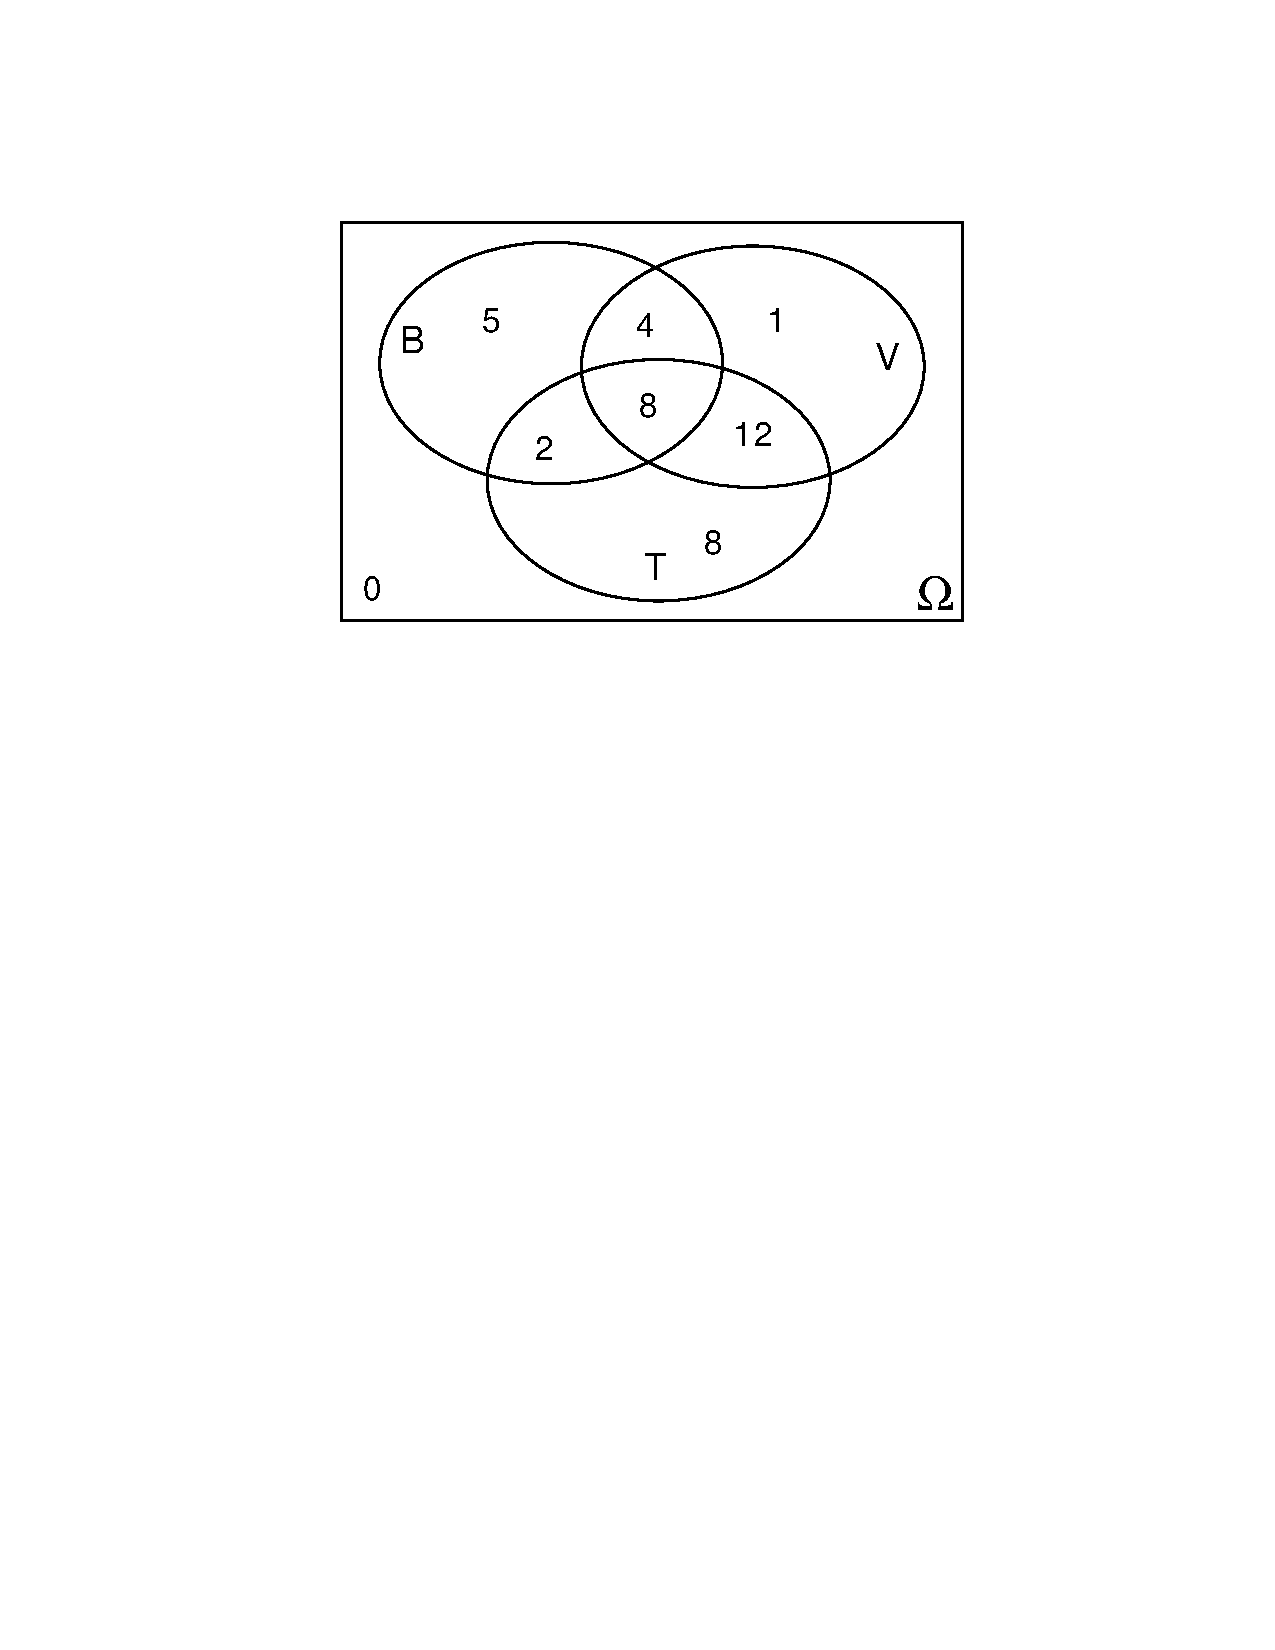
\includegraphics[width=2in]{venn-diagram}
      }
      \vspace{.2in}
    \item 5 students only play badminton.
    \item 5 + 4 + 8 + 2 = 19 students play badminton.
    \item $\frac{\textrm{\# students that play badminton}}{\textrm{total \# students}} = \frac{19}{40}$.
    \item $\frac{\textrm{\# students that play badminton and voleyball}}{\textrm{\# students that play voleyball}} = \frac{4 + 8}{25} = \frac{12}{25}$.
    \item The sample space has effectively been reduced from $\Omega$ down to $V$, where $V$ is the set of students that play voleyball. The proportion of the original 40 students that play badminton is not the same as the proportion of voleyball-playing students who play badminton.
  \end{enumerate}
}
